\chapter{Alberi decisionali per l'identificazione di IMBHs}
\label{chap:cap3}
Dopo aver introdotto gli strumenti teorici necessari, in questo Capitolo viene descritta nello specifico l'applicazione di tali concetti al problema astrofisico in questione: l'identificazione di IMBHs al centro di GCs. In particolare, in questo lavoro di tesi, si vuole predire la presenza di IMBHs al centro dei GCs utilizzando un metodo di ML interpretabile sulla base delle caratteristiche dinamiche delle MSPs presenti nelle regioni centrali degli ammassi. I modelli di ML utilizzati sono gli alberi decisionali costruiti con l'algoritmo CART (Cap. \ref{chap:cap2}). 

In primo luogo verrà brevemente descritto il codice HiGPUs utilizzato per le simulazioni a N-corpi da cui provengono i \textit{dataset} forniti all'albero decisionale. Successivamente verranno, quindi, presentati i \textit{dataset} e poi si passerà ad una descrizione generale del codice sviluppato per la predizione.

\section{Motivazioni}
Nel Capitolo \ref{chap:cap1} si è parlato dell'importanza di identificare IMBHs al centro di ammassi e delle problematiche che si riscontrano utilizzando i metodi diretti. Abbiamo visto che esse sono legate principalmente alle difficoltà osservative, in quanto misurare le dispersioni di velocità all'interno della sfera di influenza del GC richiede elevatissime risoluzioni spaziali. Inoltre, l'identificazione di una cuspide nei profili di densità e di dispersione di velocità non sempre è indice della presenza di un IMBH.
Per lo sviluppo della tesi, invece, ci si è basati su un metodo di identificazione indiretto, ovvero quello delle MSPs \cite{abbate1:paper}. Dallo studio delle informazioni dinamiche delle MSPs all'interno dei GCs, infatti, è possibile identificare indirettamente la presenza di IMBHs in ammassi. 

In questo lavoro di tesi, però, si vuole applicare un nuovo metodo in questo contesto, ovvero servirsi di un algoritmo di ML interpretabile (gli alberi decisionali) per prevedere la presenza di IMBHs al centro di GCs. La sfida, infatti, sta proprio nel voler mettere a punto un metodo identificativo nuovo per cercare di avanzare nella risoluzione di un problema astrofisico ancora così aperto. Le informazioni delle MSPs che si vogliono fornire all'algoritmo per la predizione di IMBHs sono l'accelerazione e le sue derivate rispetto al tempo: \textit{jerks} e \textit{snaps (o jounce)}. Queste quantità sono legate alle derivate dei periodi delle MSPs nell'ammasso e, di conseguenza, sarebbe possibile stimarle a partire da tali misure. Le campagne osservative, tuttavia, richiedono tempistiche di diversi anni per ottenere \textit{jerks} e \textit{snaps} con una precisione adeguata, oltre a richiedere una certa regolarità e puntualità nelle osservazioni. Pertanto, i dati osservativi necessari non sono ancora a disposizione e, per questo lavoro, ci si è serviti dei dati provenienti da un set di simulazioni a N-corpi. Inoltre, avere dati di simulazioni in tal senso è di fondamentale importanza per un futuro confronto tra dati osservati e dati teorici. \MP{NB che il training va comunque fatto su simulazioni perché anche avendo dati di jerk e snap in ammassi reali non avremmo le etichette, visto che non sappiamo quali ammassi reali siano IMBH host e quali non lo siano.}

\section{HiGPUs}
Le simulazioni a N-corpi da cui derivano i dati forniti all'algoritmo di ML per la previsione di IMBHs nei GCs sono state ottenute mediante la nuova versione del codice \textit{HermiteIntegratorGPUs (HiGPUs)} \cite{capdolspe:paper}. Si tratta di un codice ad alta precisione, adatto a simulare l'evoluzione nel tempo di sistemi di masse puntiformi che interagiscono tramite la forza newtoniana classica.

Il codice HiGPUs (disponibile gratuitamente in \cite{HiGPUs:online}) implementa un metodo di integrazione di Hermite fino al $6^{\circ}$ordine e utilizza accelerazioni, \textit{jerks} e \textit{snaps} per far avanzare le posizioni e le velocità delle stelle nel tempo.

Lo schema che segue è diviso in tre fasi: predizione, valutazione e correzione. Di seguito verranno indicate le derivate dell'accelerazione rispetto al tempo con la notazione con i punti e chiameremo indistintamente gli elementi \textit{stelle} o \textit{particelle}. Consideriamo, quindi, un sistema composto da $N$ stelle e assumiamo che l'\textit{i-esima} particella al tempo iniziale $t_{c,0}$ sia caratterizzata da posizione $\textbf{r}_{i,0}$, velocità $\textbf{v}_{i,0}$, accelerazione $\textbf{a}_{i,0}$, \textit{jerk} $\dot{\mathbf{a}}_{i, 0}$, \textit{snap} $\ddot{\mathbf{a}}_{i, 0}$, \textit{crackle} $\dddot{\mathbf{a}}_{i, 0}$ ed un \textit{time step} $\Delta t_{i,0}$. Inoltre, chiamiamo $m$ il numero
di particelle appartenenti allo stesso blocco temporale e che devono essere evolute allo stesso tempo $t_{c,0} + \Delta t_{i,0}$. I passi da seguire sono, dunque, i seguenti:
\begin{itemize}
    \item \textit{Predizione}: consiste nel calcolo di posizione, velocità e accelerazione di tutte le stelle a partire dai valori iniziali:
    \begin{equation}
\begin{aligned}
\mathbf{r}_{i, p r e d} &=\mathbf{r}_{i, 0}+\mathbf{v}_{i, 0} \Delta t_{i, 0}+\frac{1}{2} \mathbf{a}_{i, 0} \Delta t_{i, 0}^{2}+\frac{1}{6} \dot{\mathbf{a}}_{i, 0} \Delta t_{i, 0}^{3}+\\
&+\frac{1}{24} \ddot{\mathbf{a}}_{i, 0} \Delta t_{i, 0}^{4}+\frac{1}{120} \dddot{\mathbf{a}}_{i, 0} \Delta t_{i, 0}^{5} \\
\mathbf{v}_{i, p r e d} &=\mathbf{v}_{i, 0}+\mathbf{a}_{i, 0} \Delta t_{i, 0}+\frac{1}{2} \dot{\mathbf{a}}_{i, 0} \Delta t_{i, 0}^{2}+\frac{1}{6} \ddot{\mathbf{a}}_{i, 0} \Delta t_{i, 0}^{3}+\\
&+\frac{1}{24} \dddot{\mathbf{a}}_{i, 0} \Delta t_{i, 0}^{4} \\
\mathbf{a}_{i, p r e d} &=\mathbf{a}_{i, 0}+\dot{\mathbf{a}}_{i, 0} \Delta t_{i, 0}+\frac{1}{2} \ddot{\mathbf{a}}_{i, 0} \Delta t_{i, 0}^{2}+\frac{1}{6} \dddot{\mathbf{a}}_{i, 0} \Delta t_{i, 0}^{3}
\end{aligned}
\label{eq:pred}
\end{equation}
    \item \textit{Valutazione}: calcolo dell'accelerazione e delle sue derivate prima e seconda per tutte le particelle $m<N$ sulla base delle posizioni e velocità predette. Le mutue interazioni tra l'\textit{i-esima} particella e le $N-1$ rimanenti sono descritte dalle seguenti relazioni:
    \begin{equation}
\begin{aligned}
\mathbf{a}_{i, 1}=& \sum_{j=1 \atop j \neq i}^{N} \mathbf{a}_{i j, 1}=\sum_{j=1 \atop j \neq i}^{N} m_{j} \frac{\mathbf{r}_{i j}}{r_{i j}^{3}} \\
\dot{\mathbf{a}}_{i, 1}=& \sum_{j=1 \atop j \neq i}^{N} \dot{\mathbf{a}}_{i j, 1}=\sum_{j=1 \atop j \neq i}^{N}\left(m_{j} \frac{\mathbf{v}_{i j}}{r_{i j}^{3}}-3 \alpha_{i j} \mathbf{a}_{i j, 1}\right) \\
\ddot{\mathbf{a}}_{i, 1}=& \sum_{j=1 \atop j \neq i}^{N} \ddot{\mathbf{a}}_{i j, 1}=\sum_{j=1 \atop j \neq i}^{N}\left(m_{j} \frac{\mathbf{a}_{i j}}{r_{i j}^{3}}-6 \alpha \dot{\mathbf{a}}_{i j, 1}-3 \beta_{i j} \mathbf{a}_{i j, 1}\right)
\end{aligned}
\label{eq:valut}
\end{equation}
dove $\mathbf{r}_{i j} \equiv \mathbf{r}_{j, p r e d}-\mathbf{r}_{i, \text {pred}}, \mathbf{v}_{i j} \equiv \mathbf{v}_{j, \text {pred}}-\mathbf{v}_{i, \text {pred}}, \mathbf{a}_{i j} \equiv \mathbf{a}_{j, \text {pred}}-\mathbf{a}_{i, \text {pred}},$
$\alpha_{i j} r_{i j}^{2} \equiv \mathbf{r}_{i j} \cdot \mathbf{v}_{i j}, \beta_{i j} r_{i j}^{2} \equiv v_{i j}^{2}+\mathbf{r}_{i j} \cdot \mathbf{a}_{i j}+\alpha_{i j}^{2} r_{i j}^{2}$
    \item \textit{Correzione}: le posizioni e le velocità delle $m$ particelle vengono corrette per mezzo delle accelerazioni e relative derivate secondo le relazioni:
    \begin{equation}
\begin{aligned}
\mathbf{v}_{i, \text {corr}} &=\mathbf{v}_{i, 0}+\frac{\Delta t_{i, 0}}{2}\left(\mathbf{a}_{i, 1}+\mathbf{a}_{i, 0}\right)-\frac{\Delta t_{i, 0}^{2}}{10}\left(\dot{\mathbf{a}}_{i, 1}-\dot{\mathbf{a}}_{i, 0}\right)+\\
&+\frac{\Delta t_{i, 0}^{3}}{120}\left(\ddot{\mathbf{a}}_{i, 1}+\ddot{\mathbf{a}}_{i, 0}\right) \\
\mathbf{r}_{i, c o r r} &=\mathbf{r}_{i, 0}+\frac{\Delta t_{i, 0}}{2}\left(\mathbf{v}_{i, \operatorname{corr}}+\mathbf{v}_{i, 0}\right)-\frac{\Delta t_{i, 0}^{2}}{10}\left(\mathbf{a}_{i, 1}-\mathbf{a}_{i, 0}\right)+\\
&+\frac{\Delta t_{i, 0}^{3}}{120}\left(\dot{\mathbf{a}}_{i, 1}+\dot{\mathbf{a}}_{i, 0}\right)
\end{aligned}
\label{eq:correz}
\end{equation}
\end{itemize}

HiGPUs è un codice ad alta precisione perché oltre ad utilizzare l'integrazione di Hermite fino al $6^{\circ}$ ordine, calcola sempre le interazioni mutue tra tutte le stelle e definisce un \textit{time step} variabile per ciascuna stella sulla base delle loro accelerazioni. Questo garantisce un buon compromesso tra precisione e velocità di calcolo. 

Tuttavia, utilizzando intervalli temporali differenti durante l’integrazione, nel caso di incontri ravvicinati tra stelle, potrebbe accadere che l’intervallo temporale diventi così piccolo da bloccare l’integrazione \MP{come è il caso in cui si voglia simulare un ammasso stellare per la tipica vita media di uno di questi oggetti, dell'ordine dell'età dell'universo in cui si formano binarie dinamicamente importanti con periodi dell'ordine di un anno}. Per ovviare al problema si può utilizzare il \textit{softening} $\epsilon$: una costante che fa in modo che le forze di interazione ed i rispettivi potenziali vengano smorzati per piccoli \textit{$r_{i,j}$}. In questo modo, il potenziale di interazione tra due particelle di massa $m_{i}$ ed $m_{j}$ diventerà:
\begin{equation}
U_{i j}=\frac{G m_{i} m_{j}}{\sqrt{r_{i j}^{2}+\epsilon^{2}}}
\label{eq:soft}
\end{equation}

\section{Simulazioni e condizioni iniziali}
Le simulazioni da cui provengono i \textit{dataset} utilizzati, sono state effettute sul supercomputer del CINECA \cite{cineca:online} mediante l'utilizzo del codice HiGPUs.

E' stato fatto evolvere un set di ammassi stellari; nello specifico sono state utilizzate circa 200 \MP{196} simulazioni. Ogni ammasso è composto da un numero di stelle variabile fino a $N=100000$ ed è rappresentato da una funzione di distribuzione di Plummer \cite{plummer:paper}. Si tratta del modello di ammasso stellare più semplice che si possa avere \MP{Dire così è un po' eccessivo, ce ne sono altri come la sfera isoterma}. Esso è simmetrico nello spazio delle fasi ed è caratterizzato dalla distribuzione di densità:
\begin{equation}
\rho(r)=\frac{3 M}{4 \pi a^{3}}\left(1+\frac{r^{2}}{a^{2}}\right)^{-\frac{5}{2}}
\label{eq:plummer}
\end{equation}
e potenziale corrispondente:
\begin{equation}
\Phi_{P}(r)=-\frac{G M}{\sqrt{r^{2}+a^{2}}}
\end{equation}
con $G$ costante di gravitazione universale, $M$ massa totale dell'ammasso, $r$ la cordinata radiale ed $a$ lunghezza di scala (\textbf{parametri usati?}).

Le singole particelle sono state generate seguendo una funzione di massa iniziale (\textit{Initial Mass Function, IMF}) di Kroupa 2001 \cite{kroupa:paper} definita come: 
\begin{equation}
N(m) d m \propto m^{-\alpha} d m
\label{eq:kroupa}
\end{equation}
dove
\begin{equation}
\alpha=\left\{\begin{array}{lll}
0.3 & \text { se } m<0.08 M_{\odot}\\
1.3 & \text { se } 0.08<m<0.5 M_{\odot} \\
2.3 & \text { se } m>0.5 M_{\odot}
\end{array}\right.
\end{equation}
Le masse delle singole stelle variano tra un minimo fissato a $0.1M_{\odot}$ ed un massimo variabile nell'intervallo $10-100M_{\odot}$ a causa degli effetti dovuti alla presenza di un IMBH. Anche la massa centrale dell'IMBH è stata fatta variare, in questo caso tra 0 e $10^{4}M_{\odot}$. Inoltre, ogni sistema è stato simulato fino ad un tempo variabile tra \textbf{?} e \textbf{?}. Infine, le simulazioni non includono nè binarie primordiali nè evoluzione stellare.

Di seguito vengono mostrati i risultati per uno degli ammassi simulati con queste condizioni iniziali.
\begin{figure}[H]
\begin{center}
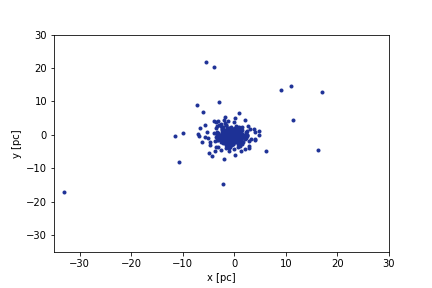
\includegraphics[width=0.5\columnwidth]{images/cluster_xy.png}
\end{center}
\caption{Proiezione di un ammasso campione sul piano del cielo.}
\label{fig:cluster}
\end{figure}
In figura \ref{fig:cluster} vi è la proiezione sul piano del cielo dell'ammasso. In figura \ref{fig:cluster1} sono riportati gli andamenti dell'accelerazione, del \textit{jerk} e dello \textit{snap} in funzione del raggio dell'ammasso. Per questi ultimi, si nota nelle regioni centrali una dispersione: probabilmente si tratta di particelle interagenti, in quanto presentano valori di accelerazione, \textit{jerk} e \textit{snap} maggiori rispetto agli andamenti generali. 
\begin{figure}[H]
\centering
\subfloat[accelerazione VS raggio]{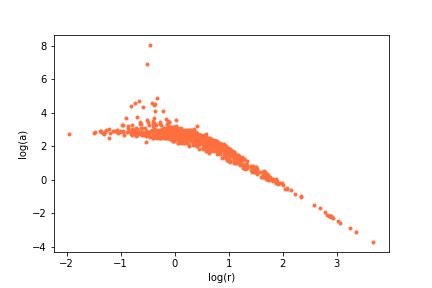
\includegraphics[width = 2.5in]{images/acc_r.png}}
\qquad
\subfloat[\textit{jerk} VS raggio]{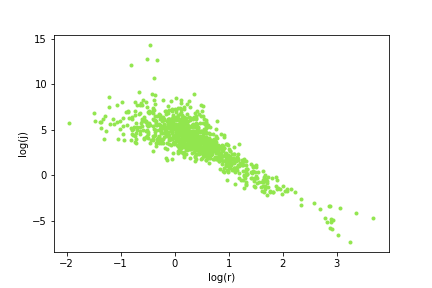
\includegraphics[width = 2.5in]{images/jerk_r.png}}
\qquad
\subfloat[\textit{snap} VS raggio]{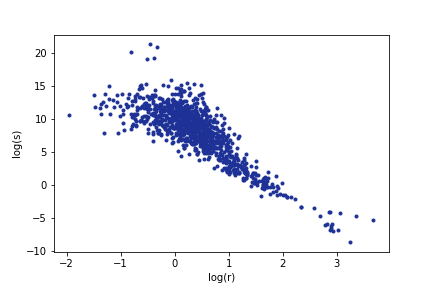
\includegraphics[width = 2.5in]{images/snap_r.png}}
\caption{Andamenti di accelerazione, \textit{jerk} e \textit{snap} in funzione del raggio delle particelle nell'ammasso campione in scala logaritmica.}
\label{fig:cluster1}
\end{figure}
In figura \ref{fig:cluster2}, invece, vi sono i \textit{jerks} e gli \textit{snaps} in funzione delle accelerazioni. Infine in figura \ref{fig:density} è riportato il profilo radiale di densità di massa dell'ammasso. Tutti i grafici sono in scala logaritmica.  
\begin{figure}[H]
\centering
\subfloat[\textit{jerk} VS accelerazione]{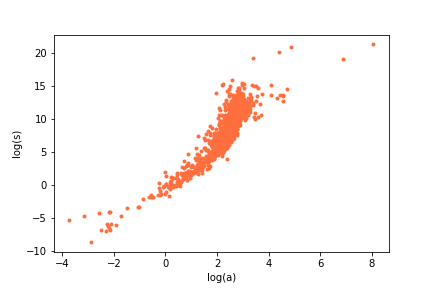
\includegraphics[width = 2.5in]{images/snap_acc.png}}
\qquad
\subfloat[\textit{snap} VS accelerazione]{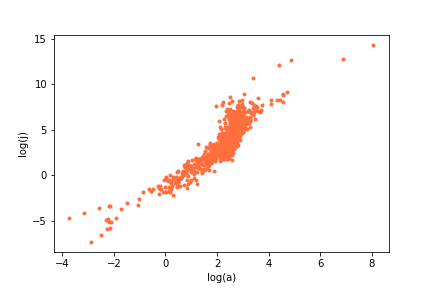
\includegraphics[width = 2.5in]{images/jerk_acc.png}}
\caption{\textit{Jerk} e \textit{snap} in funzione dell'accelerazione delle stelle dell'ammasso in scala logaritmica.}
\label{fig:cluster2}
\end{figure}
\begin{figure}[H]
\begin{center}
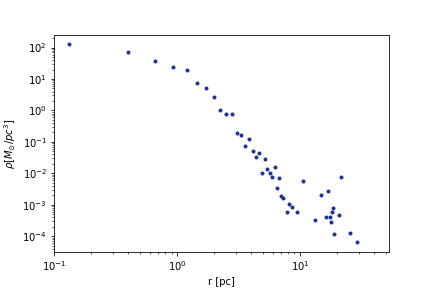
\includegraphics[width=0.5\columnwidth]{images/density.png}
\end{center}
\caption{Profilo di densità dell'ammasso in scala logaritmica.}
\label{fig:density}
\end{figure}

\section{Dataset}
Tra i risultati delle simulazioni sono stati considerati solo quelli relativi alle particelle delle zone più interne degli ammassi, in quanto, normalmente le MSPs si trovano proprio in tali regioni. 

Si è deciso di definire le zone centrali degli ammassi per mezzo del raggio che contenesse il $20\%$ delle stelle totali. Successivamente, in queste regioni, sono state eseguite 6 estrazioni casuali per ogni ammasso di un numero di MSPs variabile tra 1 e 40. Trattandosi di simulazioni che non tengono conto dell'evoluzione stellare, le particelle risultano tutte uguali, per questo motivo la scelta di estrarle casualmente è ragionevole. Tuttavia, si è scelto di selezionarle nelle regioni centrali poiché è lì che normalmente si trovano. 

I \textit{dataset} forniti all'algoritmo di ML sono in totale sei ed essi differiscono tra loro in base al diverso numero di MSPs estratte per ciascun ammasso, ovvero 1, 5, 10, 20, 30 o 40.
Pertanto, ogni \textit{record} dei diversi \textit{dataset} corrisponde ad un ammasso e, come già detto, gli ammassi simulati sono circa 200. Ciascun ammasso può contenere o meno un IMBH ed è caratterizzato da un certo numero di particelle da 1 a 40 che sono state estratte casualmente come MSPs. 

Ogni MSP è caratterizzata da posizione nell'ammasso, velocità, accelerazione, \textit{jerk} e \textit{snap}. Ma le caratteristiche delle MSPs che si è deciso di fornire come \textit{features} all'albero decisionale sono: 
\begin{itemize}
    \item il raggio proiettato sul piano del cielo, cioè la distanza di ogni particella dal centro di massa dell'ammasso: $r_{p}=\sqrt{x^{2}+y^{2}}$;
    \item la componente $z$ della velocità, $v_{z}$;
    \item la componente $z$ dell'accelerazione, $a_{z}$;
    \item la componente $z$ del \textit{jerk}, che ora indicheremo con $j_{z}$;
    \item la componente $z$ dello \textit{snap}, che indicheremo con $s_{z}$.
\end{itemize}

Sulla base di tali \textit{features} per ciascun \textit{dataset}, l'algoritmo di ML sarà in grado di predire la presenza di un IMBH negli ammassi con una certa accuratezza ed \textit{F-score}.

\section{Codice}
Il codice sviluppato per la predizione degli IMBHs al centro di GCs mediante l'utilizzo di alberi decisionali è stato scritto in Python 3.7.0 utilizzando i moduli \textbf{NumPy} \cite{numpy:online} e \textbf{scikit-learn} \cite{sklearn:online}. Esso è consultabile al seguente link di \textit{jupyter notebook}: \textbf{inserire}.

Il codice si sviluppa principalmente in quattro parti:
\begin{itemize}
    \item Fase di preparazione del \textit{dataset};
    \item Fase di addestramento sul \textit{training set};
    \item Fase di validazione;
    \item Valutazione delle prestazioni sul \textit{test set}.
\end{itemize}

Durante la prima fase, il \textit{dataset} viene diviso nei tre sottogruppi: \textit{training set}, \textit{validation set} e \textit{test set} (Sez. \ref{sec:splitdata}).
Per questo lavoro si è scelto di considerare nel \textit{test set} il $20\%$ dei dati e il restante $80\%$ viene suddiviso nel seguente modo: il $30\%$ di questi dati costituisce il \textit{validation set} ed il rimanente $70\%$ fa parte del \textit{training set}. Pertanto, il \textit{dataset} è diviso in: $56\%$ in \textit{training set}, $24\%$ in \textit{validation set} e $20\%$ in \textit{test set}. 

Nella fase successiva, l'albero decisionale di classificazione viene addestrato sul \textit{training set}. Trattandosi di un algoritmo supervisionato, quindi, gli viene fornito in input anche il vettore delle \textit{labels} in cui le due classi considerate vengono indicate con:
\begin{itemize}
    \item \textbf{classe 0 o "no"}: "non c'è un IMBH nell'ammasso";
    \item \textbf{classe 1 o "yes"}: "c'è un IMBH nell'ammasso".
\end{itemize}
Per distinguere le classi si è fissato a priori un valore di soglia per la massa. In particolare, si è decisiso di inserire nella \textbf{classe "yes"} tutti gli ammassi per cui $$\frac{M_{BH}}{M_{clus}}>0.14$$ dove con $M_{BH}$ si indica la massa del buco nero centrale e con $M_{clus}$ la massa dell'intero ammasso. Quando, invece, la massa del buco nero centrale risulta inferiore o uguale al $14\%$ della massa dell'intero ammasso, consideriamo che non ci sia un IMBH al centro dell'ammasso in questione.

Durante la fase di validazione, poi, avviene il processo di \textit{pruning} dell'albero (Sez. \ref{sec:pruning}). In questa fase si vuole scegliere il parametro di complessità $\alpha$ relativo al modello allenato per cui non si abbia \textit{overfitting}, ma che permetta di migliorare l'accuratezza delle previsioni. Come già visto in maggiore dettaglio nelle Sezioni \ref{sec:pruning} e \ref{sec:splitdata}, per ogni valore del parametro $\alpha$ che l'algoritmo fa variare in maniera crescente tra 0 e 1, esiste un'unica sottostruttura dell'albero $T$ che minimizzi la \ref{eq:costcompl}. Ad ognuno degli $\alpha$ selezionati e salvati in memoria dall'algoritmo corrisponde un modello allenato. Si vuole ora scegliere il migliore tra essi in modo da ottenere un classificatore in grado di predire in maniera accurata la presenza degli IMBHs al centro dei GCs. Per fare ciò si utilizza il \textit{validation set}. In particolare, in seguito alla fase di addestramento, il codice identifica il modello classificatore corrispondente al relativo $\alpha$ in grado di fare una predizione sul \textit{validation set} con la miglior accuratezza possibile.\\
In figura \ref{fig:acc_20part} si riporta l'andamento delle accuratezze dei modelli allenati per ciascun valore del parametro di complessità $\alpha$ in funzione del numero progressivo degli $\alpha$ stessi. Questo grafico è un esempio ottenuto a partire dal \textit{dataset} con l'estrazione di 20 MSPs per ogni ammasso, ma si è svolto lo stesso procedimento per tutti i \textit{dataset}.\\
Il modello scelto, quindi, è quello per cui si ha il massimo valore di accuratezza nelle previsioni sul \textit{validation set}.

\begin{figure}[ht]
\begin{center}
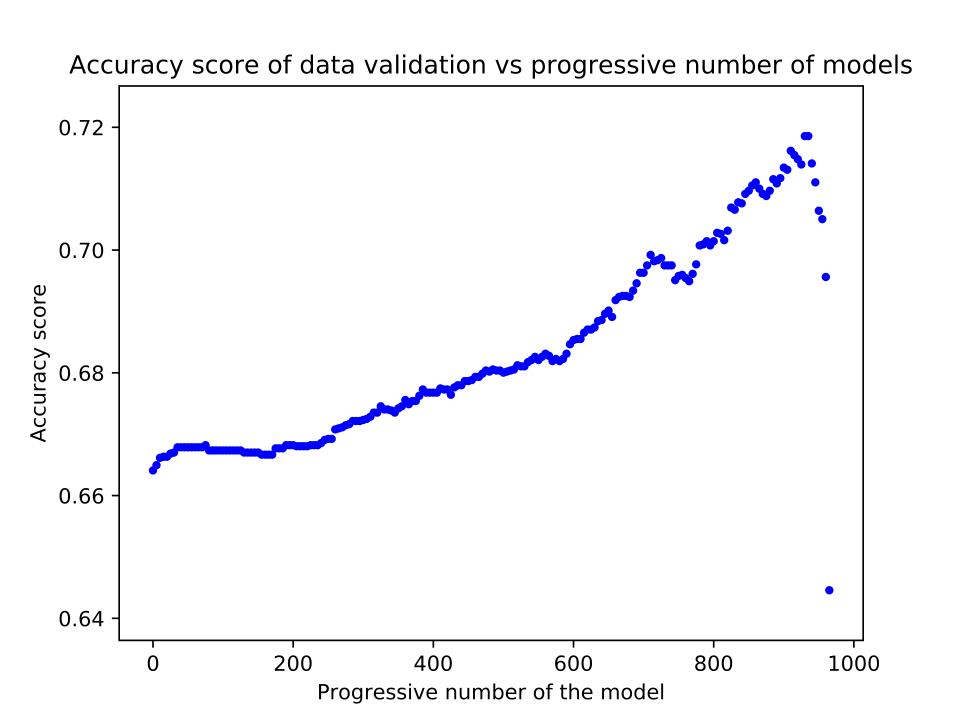
\includegraphics[width=0.7\columnwidth]{images/acc_val_20part.png}
\end{center}
\caption{Il plot è stato ottenuto a partire dal \textit{dataset} contenente 20 MSPs per ogni ammasso. Si riporta l'andamento delle accuratezze ottenute con ciascun modello allenato in funzione del numero progressivo di $\alpha$. Il modello scelto è quello che restituisce il massimo valore di accuratezza sul \textit{validation set}.}
\label{fig:acc_20part}
\end{figure}

Una volta scelto il modello, le sue prestazioni vengono valutate su un set di dati totalmente nuovi per lui: il \textit{test set}. Dopo il \textit{pruning}, infatti, il modello è in grado di classificare nuovi ammassi con una certa accuratezza senza produrre \textit{overfitting}.

